 % http://www.risc.jku.at/people/ckoutsch/stuff/e_algorithms.html

 \def \ae % 5
 {
 \begin{textarea}[]
 	\only<1>{
    \doublepic
  }
 	\only<2>{
 		This algorithm solves the single-source shortest path problem for a directed graph with nonnegative edge weights. 
 	}
 	\only<3>{
 		What is Dijkstra's algorithm?
 	}
 \end{textarea}
 }

\def \ac % 3
{
\begin{textarea}[]
	\only<1>{
		Technique for finding a particular value in a linear array by ruling out half of the data at each step.
	}
	\only<2>{
		What is Binary Search?
	}
\end{textarea}
}


\def \aa % 1
{
\begin{textarea}[]
  \only<1>{
    \begin{algorithm}[H]
      \textbf{FUNCTION} blublub(A)
      \begin{algorithmic}[1]
        \FOR {$n = size(A) \cdots 2$}
        \FOR {$i = 0 \cdots n-2$}
        \IF {$A[i] > A[i+1]$}
        \STATE Swap$(A[i],A[i+1])$
      \ENDIF
    \ENDFOR
  \ENDFOR
\end{algorithmic}
\end{algorithm}
}
\only<2>{
  What is Bubble Sort?
}
\end{textarea}
}

\def \ab % 2
{
\begin{textarea}[]
  \only<1>{
    \begin{algorithm}[H]
      \begin{algorithmic}[1]
        \WHILE {$\vert df \vert > \varepsilon $}
        \STATE $df = \text{gradientF(x)}$
        \STATE $x = x-\alpha df$
      \ENDWHILE
    \end{algorithmic}
  \end{algorithm}
}
\only<2>{
  What is Steepest Descent?
}
\end{textarea}
}


 \def \ad % 4
 {
\begin{textarea}[]
  \only<1>{
    \centering
    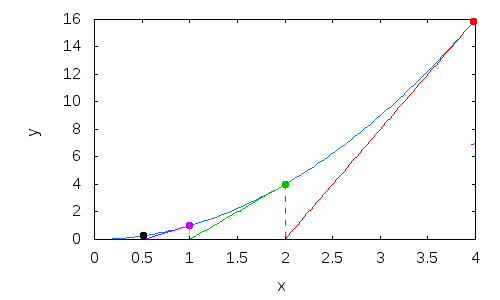
\includegraphics[height=0.5\linewidth]{../categories/media/code/Newtons_method_x2}
  }
  \only<2>{
    What is Newton's method?
  }
\end{textarea}
}
